\documentclass{article}\usepackage[]{graphicx}\usepackage[]{color}
%% maxwidth is the original width if it is less than linewidth
%% otherwise use linewidth (to make sure the graphics do not exceed the margin)
\makeatletter
\def\maxwidth{ %
  \ifdim\Gin@nat@width>\linewidth
    \linewidth
  \else
    \Gin@nat@width
  \fi
}
\makeatother

\definecolor{fgcolor}{rgb}{0.345, 0.345, 0.345}
\newcommand{\hlnum}[1]{\textcolor[rgb]{0.686,0.059,0.569}{#1}}%
\newcommand{\hlstr}[1]{\textcolor[rgb]{0.192,0.494,0.8}{#1}}%
\newcommand{\hlcom}[1]{\textcolor[rgb]{0.678,0.584,0.686}{\textit{#1}}}%
\newcommand{\hlopt}[1]{\textcolor[rgb]{0,0,0}{#1}}%
\newcommand{\hlstd}[1]{\textcolor[rgb]{0.345,0.345,0.345}{#1}}%
\newcommand{\hlkwa}[1]{\textcolor[rgb]{0.161,0.373,0.58}{\textbf{#1}}}%
\newcommand{\hlkwb}[1]{\textcolor[rgb]{0.69,0.353,0.396}{#1}}%
\newcommand{\hlkwc}[1]{\textcolor[rgb]{0.333,0.667,0.333}{#1}}%
\newcommand{\hlkwd}[1]{\textcolor[rgb]{0.737,0.353,0.396}{\textbf{#1}}}%
\let\hlipl\hlkwb

\usepackage{framed}
\makeatletter
\newenvironment{kframe}{%
 \def\at@end@of@kframe{}%
 \ifinner\ifhmode%
  \def\at@end@of@kframe{\end{minipage}}%
  \begin{minipage}{\columnwidth}%
 \fi\fi%
 \def\FrameCommand##1{\hskip\@totalleftmargin \hskip-\fboxsep
 \colorbox{shadecolor}{##1}\hskip-\fboxsep
     % There is no \\@totalrightmargin, so:
     \hskip-\linewidth \hskip-\@totalleftmargin \hskip\columnwidth}%
 \MakeFramed {\advance\hsize-\width
   \@totalleftmargin\z@ \linewidth\hsize
   \@setminipage}}%
 {\par\unskip\endMakeFramed%
 \at@end@of@kframe}
\makeatother

\definecolor{shadecolor}{rgb}{.97, .97, .97}
\definecolor{messagecolor}{rgb}{0, 0, 0}
\definecolor{warningcolor}{rgb}{1, 0, 1}
\definecolor{errorcolor}{rgb}{1, 0, 0}
\newenvironment{knitrout}{}{} % an empty environment to be redefined in TeX

\usepackage{alltt}
\usepackage{enumitem}
\usepackage{ amssymb }
\usepackage{ textcomp }
\usepackage{longtable}
\usepackage{amsmath,tabu}


\topmargin=-0.45in
\evensidemargin=0in
\oddsidemargin=0in
\textwidth=6.5in
\textheight=9.0in
\headsep=0.25in

\title{Perturb Seq}
\author{Caleb Lareau}
\date{\today}
\IfFileExists{upquote.sty}{\usepackage{upquote}}{}
\begin{document}
\maketitle

\section*{Introduction}
In three recent (December 2016) papers published  in the journal \textit{Cell}, researchers at the Broad Institute, UCSF, and the Weizmann Institute described a new technology called Perturb-Seq, which integrates CRISPR-Cas9 genome editing and droplet-based single-cell RNA-Seq. \textbf{Figure \ref{fig:overview}} provides a graphical overview of this technology. 

\begin{figure}[ht]
    \centering
    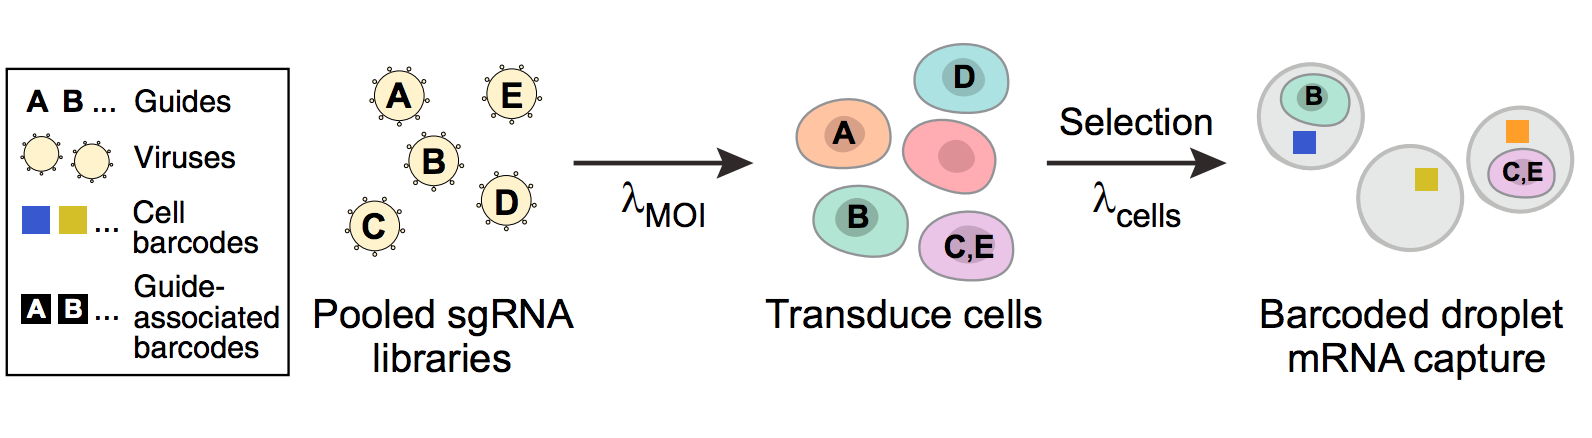
\includegraphics[width=\textwidth]{overview.png}
    \caption{\textbf{A graphical overview of the experimental design of Perturb-Seq.} In brief, viruses containing different genome-editing vectors (labeled \textbf{A,B,C,D,E}) infect cells and then modify the host cells' DNA using CRISPR/Cas-9. These modified cells are then experimentally examined using a high-throughput microfluidics droplet-based capture. The result of this experiment are data with a complex correlation structure that I propose to be examined further.
    \label{fig:overview}}
\end{figure}

\noindent \textbf{The basic idea is to knock-out (``Perturb'') certain key regulators} (equivalently, genes or transcription factors) in a cell and \textbf{then examine how the cell responds to these changes.} The cellular response is measured through RNA-\textbf{Sequencing}, hence the name of the technology. Though the biological underpinnings of Perturb-Seq in itself is not new, the \textbf{sample size} ($> 200,000$) and \textbf{resolution} (single cell) distinguish this method from all other existing technologies. In essence, Perturb-Seq is doing thousands of carefully controlled experiments in parallel, enabling an unprecedented throughput of experimental data. Early review articles have suggested that Perturb-Seq could be \textbf{the key technology for dissecting gene regulation in the context of disease}. So far, only a handful of primarily biologically-motivated folk have begun to think about modeling these very complicated data. \textbf{The goal of this project, thus, is to 1) convey the importance and theory of this experimental data source, 2) discuss existing modes of estimation/inference, and 3) situate the analyses problems in the context of discussion of BST 245}.

\label{fig:model} 

\begin{figure}[ht]
    \centering
    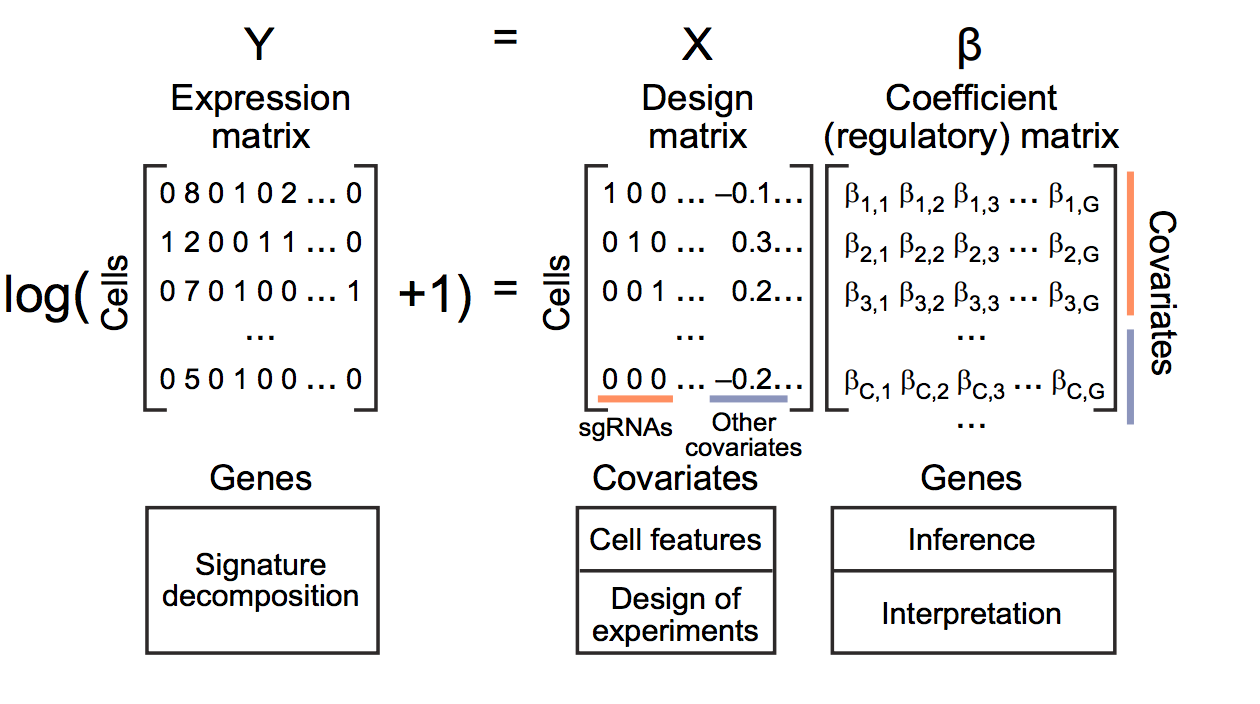
\includegraphics[width=\textwidth]{model.png}
    \caption{\textbf{A graphical overview of the generalized linear model fit in Perturb-Seq analyses.}}
     \label{fig:model}
\end{figure}


\section*{State of the stats}
Atray Dixit maintains a Github repository (https://github.com/asncd/MIMOSCA), which contains a python script with about 2,000 lines of code that defines the backbone of the statistical methodology for Perturb-Seq. In brief, this code base fits an elastic net linear model to a design matrix and gene expression readout as depicted in \textbf{Figure \ref{fig:model}}. Of note, the dimensions for this analysis will be on the order of $50,000$ cells, $30,000$ genes, and $50$ covariates. \textbf{There is no existing infrastructure to examine this data in \texttt{R}, which will be a component of the ``resource" uility in the proposed project}. The aim/expectation is that ``translating'' the presentation of the data from the authors into a format more typically consumed by the Biostastics department will expedite statistical innovation that is direly needed for this data type. 

\section*{Links to the BST245 Course}
\begin{itemize}
  \item Repeated measurements (the same cell/sgRNA combination is detected $\sim$ 500 times)
  \item Correlated independent variables (effects of sgRNAs may be correlated if they underlie the same regulatory process)
  \item Correlated dependent variables (gene RNA values are inherently highly correlated)
\end{itemize}

\section*{Presentation Outline}
\begin{itemize}
  \item 0-7 minutes: Discussion of CRISPR/Cas9, scRNA-Seq, Drop-Seq, and gene regulation
  \item 7-12 minutes: Discussion of Perturb-Seq
  \item 12-15 minutes: Key takeaways of the Perturb-Seq paper as presented
  \item 15-20 minutes: Translating between Perturb-Seq and BST245 Notations
  \item 20-25 minutes: High-level exploratory data analysis 
  \item 25-32 minutes: Discussion of model fits previously implemented
  \item 32-38 minutes: Analysis of model fits, coefficients, etc. 
  \item 38-40 minutes: Immediate recommendations for improvement of statistical models
  \item 40-50 minutes: Discussion 

  
\end{itemize}


\section*{References}
Adamson, Britt, et al. ``A multiplexed single-cell CRISPR screening platform enables systematic dissection of the unfolded protein response." Cell 167.7 (2016): 1867-1882. \newline \newline
Dixit, Atray, et al. ``Perturb-seq: dissecting molecular circuits with scalable single-cell RNA profiling of pooled genetic screens." Cell 167.7 (2016): 1853-1866. \newline \newline
Jaitin, Diego Adhemar, et al. ``Dissecting Immune Circuits by Linking CRISPR-Pooled Screens with Single-Cell RNA-Seq." Cell 167.7 (2016): 1883-1896. \newline \newline
Wagner, Daniel E., and Allon M. Klein. ``Genetic screening enters the single-cell era." Nature Methods 14.3 (2017): 237-238.
\end{document}
